\chapter{Sonstige Distributed-Ledger-Technologie}
\section{Directed Acyclic Graph}
Bei einem DAG handelt es sich um eine gerichteten azyklischen Graphen, der im Bereich der  Distributed-Ledger-Technologie dazu eingesetzt wird Transaktionen zu speichern.
Die Kryptowährung IOTA\footnote{\url{https://www.iota.org/}} setzt solch eine Datenstruktur ein. Der Konsens entsteht nicht durch eine Blockchain auf die sich alle Teilnehmer mithilfe des Konsensalgorithmus einigen. Der Konsens entsteht dadurch, dass Teilnehmer neue Transaktionen nur auf Transaktionen aufbauen, die sie für gültig halten. Um eine Transaktion in den Graphen zu schreiben, muss der Absender Proof-of-Work erledigen.

\begin{figure}[H]
\centering
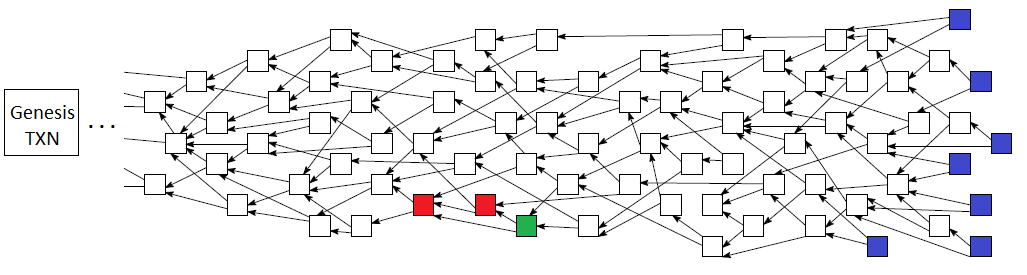
\includegraphics[width=1\linewidth]{Figures/tangle}
\decoRule
\caption{Directed Acyclic Graph}
\label{fig:tangle}
\end{figure}

Die grüne Transaktion aus Abbildung \ref{fig:tangle} baut auf den beiden roten Transaktionen auf und bestätigt diese auf diese Art und Weise. Je tiefer eine Transaktion im Graphen steckt, desto mehr Proof-of-Work baut auf ihr auf. Am rechten Rand befinden sich in blau neue, unbestätigte Transaktionen.\\\\
Kryptowährungen auf Basis solch einer Datenstruktur sind nicht für die Gewinnerauswahl einer Glücksspielanwendung nutzbar, da man sich nicht bereits im Vorfeld auf ein eindeutiges, in der Zukunft liegendes, aber dennoch zufälliges Ereignis einigen kann. Weiterführende Informationen zu IOTA und eine genaue Beschreibung der DAG Datenstruktur findet man in \cite{tangle_whitepaper}.


\section{Proof of Stake }\label{pos}
%Bei Proof of Stake handelt es sich um einen Konsensalgorithmus...Die grundlegende Idee von Proof of Stake ist es, dass die Teilnehmer des Netzwerks über den nächsten Block abstimmen. 
Proof of Stake bezeichnet ein Konsensalgorithmus mit dem ein Blockchain-Netzwerk sich durch einen gewichteten Zufallswert darauf einigt, welcher Teilnehmer den nächsten Block erzeugen darf. Je höher die Anzahl Kryptowährungseinheiten (der sogenannte Stake\footnote{Der Stake ist somit der Anteilsnachweis, der dem Teilnehmer einen Anreiz verleihen soll, sich der Konsensregeln entsprechend zu verhalten. Je nach Implementierung fließen auch noch andere Werte wie beispielsweise die Teilnahmedauer (Coin-Age) in die Berechnung ein.}) eines Teilnehmers, desto höher ist die Wahrscheinlichkeit, dass dieser den nächsten Block bestimmen darf. Solch ein Abstimmungsprozess ist deutlich Ressourcen schonender, da die beim Mining(Proof-of-Work) anfallenden Strom- und Hardwarekosten wegfallen. Proof of Stake hat jedoch auch einige Nachteile und ist deutlich komplexer zu implementieren. Beispielsweise ist die zufällige Auswahl des Teilnehmers, der den nächsten Block erzeugen darf, kein triviales Problem. Es gibt eine Reihe an unterschiedlichen Implementierungen des Proof of Stake Konsensalgorithmus. Die Kryptowährungen Cardano \cite{coin_ada}, NXT \cite{coin_nxt} und Peercoin \cite{coin_peercoin} verwenden Formen von Proof of Stake. Eine Reihe von Vor- und Nachteilen von Proof of Stake, sowie eine Beschreibung des Nothing-at-Stake Angriffs\footnote{Dieser Angriff beschreibt das Problem, dass Teilnehmer an mehreren Forks der Blockchain gleichzeitig arbeiten können, ohne das dadurch für sie Kosten wie beim Proof-of-Work Mining anfallen.} findet sich in \cite{proof_of_stake}.\\\\
%Es muss darauf geachtet werden, dass neue Teilnehmer, die die Blockchain vom Genesis Block aus validieren auch nachvollziehen können, dass der Teilnehmer das recht hatte den Block 
%Die Reichen werden reicher, da diese mit einer höheren Wahrscheinlichkeit den nächsten Block bestimmen dürfen und somit öfter die darin enthaltenen Transaktionsgebühren erhalten. 
Eine ausschließliche auf Proof of Stake aufbauende Kryptowährung ist nicht für die Implementierung der Zufallsauswahl einer Glücksspielanwendung geeignet. Der Teilnehmer, der den nächsten Block bestimmt, kann im Vorhinein prüfen, wie er diesen erzeugen muss, damit ein für ihn günstiges Resultat entsteht.

\section{Second Layer Solutions}
Second Layer Solutions nennt man Protokolle und Plattformen, die es ermöglichen den Base Layer (die Blockchain), möglichst wenig zu belasten, indem Transaktionen nur in die Blockchain geschrieben werden, wenn es nicht anderes möglich ist. Ein Handelsplatz auf dem man Bitcoins an- und verkaufen kann, ist ein Beispiele für eine Plattform als Second Layer Solution. Alle Transaktionen zwischen den Kunden, innerhalb des Handelsplatz, berühren nicht die Blockchain. Es werden ausschließlich Transaktionen in die Blockchain geschrieben, wenn Kunden in den Handelsplatz ein- und auszahlen. In dieser Art der Second Layer Solution nimmt der Handelsplatz die Rolle einer Trusted Third Party ein. Das Lightning Netzwerk Protokoll ist hingegen eine Second Layer Solution, das sogenannte Payment Channels verwendet, um vollständig ohne Trusted Third Party auszukommen.

%Jeder Teilnehmer, der Transaktionen validieren möchte, muss die gesamte Transaktionshistorie der Blockchain speichern. 
%Da man für das validieren der Transaktionen keine monetäre Belohnung wie den Blockreward erhält, führt eine große Blockchain zu einer Einstiegsbarriere und somit zwangsläufig zu Zentralisierung.

\subsection{Payment Channel}

Ein Payment Channel ist eine Technik, die es erlaubt eine Reihe von Zahlungen zwischen zwei Parteien auszuführen, ohne das dabei alle Zahlungstransaktionen in die Blockchain geschrieben werden müssen. Lediglich das Öffnen und Schließen eines Payment Channels erfordert Transaktionen, die in die Blockchain geschrieben werden. Alle Transaktionen auf die sich beide Teilnehmer zwischen der öffnenden und der schließenden Transaktion einigen, berühren nicht die Blockchain und werden lediglich Off-Chain ausgetauscht. Eine genaue Beschreibung, wie Payment Channels technisch funktionieren und warum keine Partei die jeweils Andere betrügen kann, findet man in \cite{lightning_white_paper}.

\subsection{Lightning Netzwerk}

Das Lightning Netzwerk umfasst circa 2000 Netzwerkknoten, die mit über 6000 Payment Cannel miteinander verbunden sind \cite{lightning_explorer}. \todo{Reicht es in der Quelle das Datum anzugeben oder muss ich auch explizit nochmal schreiben: Stand Ende Main 2018} Es erlaubt Off-Chain Zahlungen zwischen den Teilnehmern, auch wenn diese nicht direkt über einen Payment Cannel miteinander verbunden sind.\footnote{Dies funktioniert unter der Voraussetzung, dass ein Pfad aus Payment Channel existiert, der beide Teilnehmern verbindet.} \\\\
Die Bitcoin Glücksspielanwendung aus Kapitel \ref{btc} könnte Off-Chain Transaktionen über das Lightning Netzwerk für Ein- und Auszahlungen akzeptieren. Diese würden Transaktionskosten für die Teilnehmer deutlich reduzieren. Off-Chain Transaktionen sind allerdings nicht für alle Teilnehmer des Spiels nachprüfbar, da sie nicht in die Blockchain geschrieben werden. Die Anforderung der transparenten Ein- und Auszahlungen wäre somit verletzt.